%%%%%%%%%%%%%%%%%%%%%%%%%%%%% Define Article %%%%%%%%%%%%%%%%%%%%%%%%%%%%%%%%%%
\documentclass{article} 
%%%%%%%%%%%%%%%%%%%%%%%%%%%%%%%%%%%%%%%%%%%%%%%%%%%%%%%%%%%%%%%%%%%%%%%%%%%%%%%

%%%%%%%%%%%%%%%%%%%%%%%%%%%%% Using Packages %%%%%%%%%%%%%%%%%%%%%%%%%%%%%%%%%%
\usepackage{geometry}
\usepackage{graphicx}
\usepackage{amssymb}
\usepackage{amsmath}
\usepackage{amsthm}
\usepackage{empheq}
\usepackage{mdframed}
\usepackage{booktabs}
\usepackage{lipsum}
\usepackage{graphicx}
\usepackage{color}
\usepackage{psfrag}
\usepackage{pgfplots}
\usepackage{bm}
\usepackage{hyperref}
%%%%%%%%%%%%%%%%%%%%%%%%%%%%%%%%%%%%%%%%%%%%%%%%%%%%%%%%%%%%%%%%%%%%%%%%%%%%%%%

% Other Settings

%%%%%%%%%%%%%%%%%%%%%%%%%% Page Setting %%%%%%%%%%%%%%%%%%%%%%%%%%%%%%%%%%%%%%%
\geometry{a4paper}

%%%%%%%%%%%%%%%%%%%%%%%%%% Define some useful colors %%%%%%%%%%%%%%%%%%%%%%%%%%
\definecolor{ocre}{RGB}{243,102,25}
\definecolor{mygray}{RGB}{243,243,244}
\definecolor{deepGreen}{RGB}{26,111,0}
\definecolor{shallowGreen}{RGB}{235,255,255}
\definecolor{deepBlue}{RGB}{61,124,222}
\definecolor{shallowBlue}{RGB}{235,249,255}
%%%%%%%%%%%%%%%%%%%%%%%%%%%%%%%%%%%%%%%%%%%%%%%%%%%%%%%%%%%%%%%%%%%%%%%%%%%%%%%

%%%%%%%%%%%%%%%%%%%%%%%%%% Define an orangebox command %%%%%%%%%%%%%%%%%%%%%%%%
\newcommand\orangebox[1]{\fcolorbox{ocre}{mygray}{\hspace{1em}#1\hspace{1em}}}
%%%%%%%%%%%%%%%%%%%%%%%%%%%%%%%%%%%%%%%%%%%%%%%%%%%%%%%%%%%%%%%%%%%%%%%%%%%%%%%

%%%%%%%%%%%%%%%%%%%%%%%%%%%% English Environments %%%%%%%%%%%%%%%%%%%%%%%%%%%%%
\newtheoremstyle{mytheoremstyle}{3pt}{3pt}{\normalfont}{0cm}{\rmfamily\bfseries}{}{1em}{{\color{black}\thmname{#1}~\thmnumber{#2}}\thmnote{\,--\,#3}}
\newtheoremstyle{myproblemstyle}{3pt}{3pt}{\normalfont}{0cm}{\rmfamily\bfseries}{}{1em}{{\color{black}\thmname{#1}~\thmnumber{#2}}\thmnote{\,--\,#3}}
\theoremstyle{mytheoremstyle}
\newmdtheoremenv[linewidth=1pt,backgroundcolor=shallowGreen,linecolor=deepGreen,leftmargin=0pt,innerleftmargin=20pt,innerrightmargin=20pt,]{theorem}{Theorem}[section]
\theoremstyle{mytheoremstyle}
\newmdtheoremenv[linewidth=1pt,backgroundcolor=shallowBlue,linecolor=deepBlue,leftmargin=0pt,innerleftmargin=20pt,innerrightmargin=20pt,]{definition}{Definition}[section]
\theoremstyle{myproblemstyle}
\newmdtheoremenv[linecolor=black,leftmargin=0pt,innerleftmargin=10pt,innerrightmargin=10pt,]{problem}{Problem}[section]
%%%%%%%%%%%%%%%%%%%%%%%%%%%%%%%%%%%%%%%%%%%%%%%%%%%%%%%%%%%%%%%%%%%%%%%%%%%%%%%

%%%%%%%%%%%%%%%%%%%%%%%%%%%%%%% Plotting Settings %%%%%%%%%%%%%%%%%%%%%%%%%%%%%
\usepgfplotslibrary{colorbrewer}
\pgfplotsset{width=8cm,compat=1.9}
%%%%%%%%%%%%%%%%%%%%%%%%%%%%%%%%%%%%%%%%%%%%%%%%%%%%%%%%%%%%%%%%%%%%%%%%%%%%%%%

%%%%%%%%%%%%%%%%%%%%%%%%%%%%%%% Title & Author %%%%%%%%%%%%%%%%%%%%%%%%%%%%%%%%
\title{Tarea 4: Backpropagation}
\author{Leonel Guerrero}
%%%%%%%%%%%%%%%%%%%%%%%%%%%%%%%%%%%%%%%%%%%%%%%%%%%%%%%%%%%%%%%%%%%%%%%%%%%%%%%

\begin{document}
\maketitle


\section{Multilayer Perceptron with Backpropagation (MLP-BP)}

\subsection{Enunciado}
Implemente su propio perceptron multicapas para que tenga una capa oculta con un numero n de neuronas en la capa oculta y k neuronas en la capa de salida. n y k son parámetros de su red (función). Usted puede emplear el lenguaje de programación de su preferencia. Entregar el código con una documentación mínima

\subsection{Implementación}

\begin{itemize}
  \item \href{https://github.com/LeoGCode/Tarea-4--Backpropagation}{Github}
  \item \href{https://colab.research.google.com/drive/1c8swOFZ_sL5bQSOi91ajNDod2Arv-0x6?usp=sharing}{Google Colab}
\end{itemize}

\section{Prueba sobre datos}

\subsection{Enunciado}
Para los conjuntos de entrenamiento usado  en la tarea del perceptron y en el Adaline, evalué un perceptron multicapas. Evalué y compare este algoritmo con los resultados obtenidos en la tarea anterior. Comente sobre su escogería en los parámetros de aprendizaje y la arquitectura requerida para la mejor convergencia

\subsection{Evaluación y comparación del algoritmo}

Veamos primeramente las gráficas del error cuadrático medio para los conjuntos de entrenamiento y los conjunto de validación obtenidos de los archivos EarthSpace.csv, MedSci.csv y LifeSci.csv, Agri.csv para el perceptron multicapas con 1 capa oculta de 3 neuronas y 1 capa de salida de 2 neurona:

\begin{figure}[!h]
  \begin{minipage}[b]{0.45\textwidth}
    \centering
    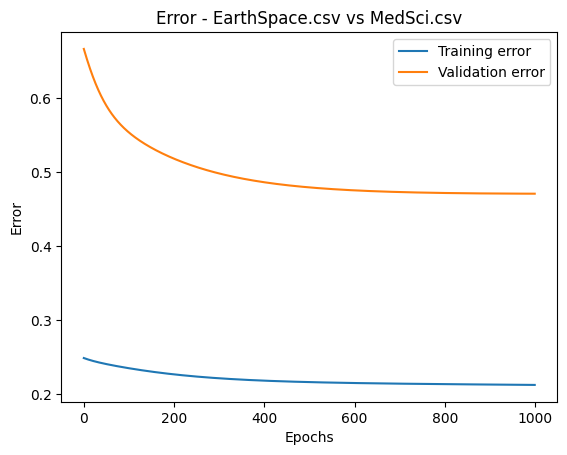
\includegraphics[width=0.95\textwidth]{./img/output.png}
    \label{fig:1}

  \end{minipage}
  \begin{minipage}[b]{0.45\textwidth}
    \centering
    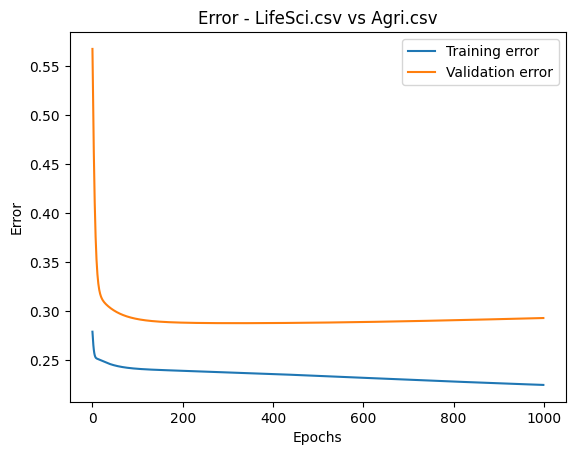
\includegraphics[width=0.95\textwidth]{./img/output2.png}
    \label{fig:2}
  \end{minipage}
  \caption{Error cuadrático medio para el conjunto de entrenamiento y el conjunto de validación para el perceptron multicapas con 1 capa oculta de 3 neuronas y 1 capa de salida de 2 neurona}
\end{figure}

\newpage
Se puede  apreciar que el error cuadrático medio para los conjuntos de entrenamiento y para los conjuntos de validación va disminuyendo a medida que se va realizando el entrenamiento. Esto es un indicador de que el algoritmo está convergiendo. De igual forma se puede ver que las curvas de error cuadrático medio para el conjunto de entrenamiento y para el conjunto de validación se encuentran muy cercanas, lo que indica que el algoritmo no está sobreajustando (overfitting) los datos.

Veamos la siguiente tabla para comparar los resultados obtenidos para el MLP contra el Adeline

\begin{table}[!h]
  \centering
  \begin{tabular}{lll}
    \cline{2-3}
                         & \multicolumn{2}{l}{Error cuadratico medio}               \\ \cline{2-3}
                         & MLP                                        & Adeline     \\ \hline
    EarthSpace vs MedSci & $2.51x10^{-5}$                             & $117.6796$  \\ \hline
    LifeScy vs Agri      & $9.21x10^{-7}$                             & $1292.4977$ \\ \hline
  \end{tabular}
\end{table}

Se puede apreciar por medio de la tabla que el MLP obtuvo mejores resultados que el Adeline. Obteniendo un error mas pequeño para los conjuntos de entrenamiento y de validación. Sin embargo cabe destacar que los datos de entrenamiento para el MLP se le aplico una transformación en contraposición al adeline que se le pasaron las datos sin ningún tipo de tratamiento

El tratamiento realizado fue el de la normalización, en el cual se le aplico la siguiente formula a cada dato de entrada:

\begin{equation*}
  x_{norm} = \frac{x - \mu}{\sigma}
\end{equation*}

Donde $\mu$ es la media de los datos y $\sigma$ es la desviación estándar de los datos. Esto se realizo para que los datos de entrada tenga una distribución normal y asi poder obtener mejores resultados. La Inicialización de los pesos se realizo tomando valores aleatorias de la distribución normal con media 0 y desviación estándar 1.

Para el MLP se escogió una taza de aprendizaje de 0.001 ya que en diferentes experimentos y tomando como referencia los pesos utilizados en el Adeline se escogió esa taza como la que mejor resultados daba. Para la arquitectura de la red se escogió una capa oculta de 3 neuronas y una capa de salida de 2 neuronas. Esto se escogió ya que en diferentes experimentos se observo que con esa arquitectura se obtuvieron mejores resultados que con otras arquitecturas.

Aparte también se escogió un valor de momentum para aumentar la velocidad de convergencia. El valor de momentum escogido fue de 0.2. Esto se escogió ya que en diferentes experimentos se observo que con ese valor se obtuvieron mejores resultados que con otros valores de momentum.


\section{Expert machine}

\subsection{Enunciado}

Considere una maquina compuesta por $K$ expertos. La función de entrada y salida del k-ésimo experto está dada por $F_k(x)$, donde $x$ es el vector de entrada y $k = 1,2, ... , K$. Las salidas individuales de los expertos están linealmente combinadas para formar la salida general y, definida por
\begin{equation*}
  y = \sum_{k=1}^{K}w_kF_k(x)
\end{equation*}
donde $w_k$ es el peso lineal asignado a $F_k(x)$. El requerimiento es evaluar $w_k$ tal que $y$ resulte ser el estimado de mínimos cuadrados de la respuesta deseada $d$ según $x$. Dado un conjunto de entrenamiento ${(x_i, d_i)}_{i=1}^N$, determine los valores requeridos de los $w_k$ para resolver este problema de estimación de parámetros.

\subsection{Respuesta}

El objetivo es encontrar los valores de los pesos $w_k$ que minimizan el error cuadrático medio entre la salida de la máquina y la salida deseada, dada por:

\begin{equation*}
  E(w) = \frac{1}{2}\sum_{i=1}^{N}(y_i - d_i)^2
\end{equation*}

donde $y_i$ es la salida de la máquina para la entrada $x_i$, y $d_i$ es la salida deseada correspondiente.

Podemos encontrar los valores de $w_k$ que minimizan $E(w)$ tomando la derivada de $E(w)$ con respecto a cada peso $w_k$ y estableciéndolos en cero:

\begin{align*}
  \frac{\partial E}{\partial w_k} & = \sum_{i=1}^{N}(y_i - d_i)\frac{\partial}{\partial w_k}\left(\sum_{j=1}^{K}w_jF_j(x_i)\right) \
                                  & = \sum_{i=1}^{N}(y_i - d_i)F_k(x_i) \
                                  & = \sum_{i=1}^{N}(w_1F_1(x_i) + w_2F_2(x_i) + ... + w_kF_k(x_i) + ... + w_KF_K(x_i) - d_i)F_k(x_i) \
                                  & = \sum_{i=1}^{N}(y_i - d_i)F_k(x_i)
\end{align*}

Igualando esto a cero, obtenemos:

\begin{equation*}
  \sum_{i=1}^{N}(y_i - d_i)F_k(x_i) = 0
\end{equation*}

Lo que nos da la ecuación para el peso $w_k$:

\begin{equation*}
  w_k = \frac{\sum_{i=1}^{N}d_iF_k(x_i)}{\sum_{i=1}^{N}F_k(x_i)^2}
\end{equation*}

Por lo tanto, para encontrar los valores de $w_k$ que minimizan el error cuadrático medio, debemos calcular las sumas $\sum_{i=1}^{N}d_iF_k(x_i)$ y $\sum_{i=1}^{N}F_k(x_i)^2$ para cada $k$, y utilizarlos en la fórmula anterior



\end{document}